%FILE: polygon.tex

\chapter{Ice Element Polygon}

\section{Introduction}

Each ice element is represented by simple convex polygon. Siku core
accepts polygons with many precomputed values described in this
chapter. Thus, all following computations are performed on Python side
of the model.

Initially, the polygon is given as a set of its extrinsic Cartesian
coordinates in Global Frame. If the coordinates are given in
Geographic coordinates, they are recalculated to extrincsic Cartesian
coordinates using~\eqref{eq:extrinsic}. Thus, we just suppose here
that all vertices are given in Global frame as a set of extrinsic
Cartesian radius-vectors: $\{\pnt{p}_j\}$, $j=0,1,\dots N-1$, total
$N$ vertices.

\section{Center of Mass, Area, Moment of Inertia}

The center of mass $\pnt{c}$ (CM) is a center of local Frame. Given
coordinates of vertices, the center of mass is calculated in
assumption that the polygon is flat. Otherwise, complicated
intergration would be necessary to accurate computations.

First, we introduce geometrical pseudo-center $\pnt{q}$ by a formula:
\begin{equation}
  \pnt{q} = \sum_{j} \pnt{p}_j / N.
\end{equation}
Although, it is not a CM, it is a convenient point that resides inside
the polygon and allows to split it in triangles as shown in
Fig.~\ref{fig:polygon}.
\begin{figure}
  \center
  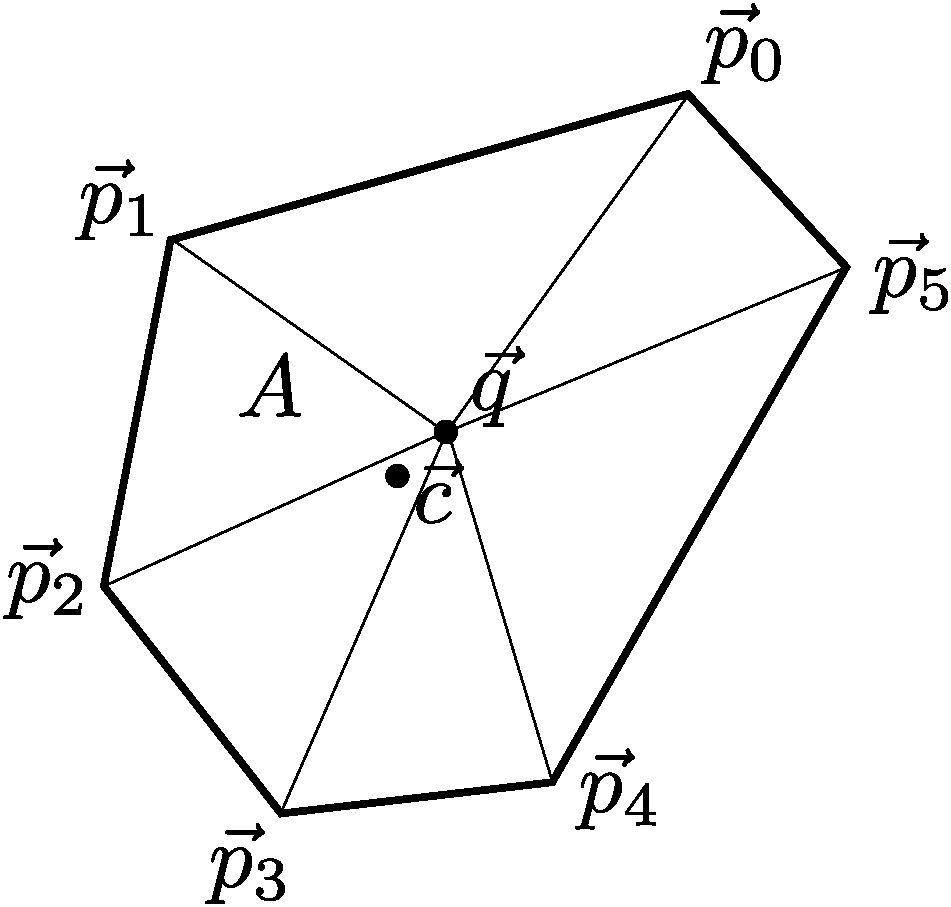
\includegraphics[width=0.35\textwidth]{pics/polygon.pdf}
  \caption{Polygon main properties computations}
  \label{fig:polygon}
\end{figure}

Now we can calculate the centers of mass of each triangle as
\begin{equation}
  \pnt{c}_i = ( \pnt{p}_i + \pnt{p}_{(i+1)'} + \pnt{q} ) / 3, \qquad
  (i+1)' = (i+1)\bmod N.
\end{equation}
And areas $A_i$ of each triangle and total area $A$.
\begin{equation}
  A_i = |(\pnt{p}_i - \pnt{q})\times (\pnt{p}_{(i+1)'} -
  \pnt{q})|,\qquad
  A = \sum_{i=0}^{N-1} A_i.
\end{equation}
Now, the center of mass can be computed as a sum of area-weighted
center of masses for each triangles:
\begin{equation}
  \pnt{c} = \sum_{i=0}^{N-1} A_i\pnt{c}_i / A.
\end{equation}
Total geometric moment of inertia (it is a moment of inertia divided
by mass) around center of mass is computed by same weighted approach:
\begin{equation}
  I/m = \sum_{i=0}^{N-1} A_i \left( (\pnt{p}_i-\pnt{c})^2 + 
  (\pnt{p}_{(i+1)'}-\pnt{c})\cdot (\pnt{p}_i-\pnt{c}) +
  (\pnt{p}_{(i+1)'}-\pnt{c})^2\right ) / (6A).
\end{equation}

\section{Mass}

Total mass need to be calculated up to at each timestep using the ice
thickness distribution function $g(h)$. General formula is
\begin{equation}
  m = \sum_{k=0}^{K-1} g(h_k) h_k\rho_k A,
\end{equation}
where $\rho_k$ is the density of ice of thickness $h_k$.
